\section*{Implementation}

FALDO is a small OWL2 ontology which fits in the ALCQ(D) classification difficulty.
It has 14 classes of which 9 deal with the concept of a Position on a sequence. 
4 of those classes there to describe accurately an what we know of a position that is not precisely determined. 
4 are to deal with the concept of a position on a strand of DNA i.e. positive, negative and on both strands.

The ontology contains only one datatype property: $faldo:position$ which is there to give a integer, one based offset from 
the start of the reference sequence. This $faldo:position$ together with the $faldo:reference$ object property links the concept
of a $faldo:Position$ to an instance of sequence in the biological sense.





FALDO was implemented and used in a number of tools and databases.

\begin{description}
\item[JBrowse sparql] FALDO is used sparql queries determine where to draw information related to a reference sequence in tracks filled with data from semantic databases. 
\item[INSDC-DDBJ] DDBJ is currently working on a RDF format for the INSDC data that is stored in DDBJ/GenBank/EMBL-Bank.
\item[BioInterchange] uses FALDO to make position information in current bioinformatics data stored in files such as GFF3 and GVF available to the semantic web\url{http://www.biointerchange.org/}.
\item[TogoGenomes] a bacterial genome database collection provided by the DBCLS also uses FALDO in its RDF representation \url{http://togogenome.org/}.
\item[Intermine] The popular model organism database software collection uses FALDO in its SPARQL mode.
\item[phenomebrowser] Positions of phenotypes and disease related natural variations are positioned onto the Mouse genome using FALDO.
\item[ENSEMBL-R2RML] The open source conversion layer to make the ENSEMBL mysql databases available on the semantic web also uses FALDO to describe all feature locations.
\item[SPARQL-bed] This simple tool that turns any BED file into a web accessible SPARQL endpoint also uses FALDO to describe BED feature positions.
\item[BioBerl] BioPerl\cite{BioPerl2002} now includes a FALDO exporter (Bio::FeatureIO::faldo), which allows any bioperl feature format to be translated to FALDO.
\item[UniProt] UniProt annotates many protein features and sites. From release 2013$\_$10 in the RDF rendering of UniProt this is done with FALDO.
\end{description}




Some tech stuff here, for example we use one-based counting
with respect to the reference sequence's forward strand
(where the reference is a nucleotide sequence).

Probably a good place to talk about strand representations?
See Figure~\ref{fig:strands}.

\begin{figure}[p]
\begin{center}
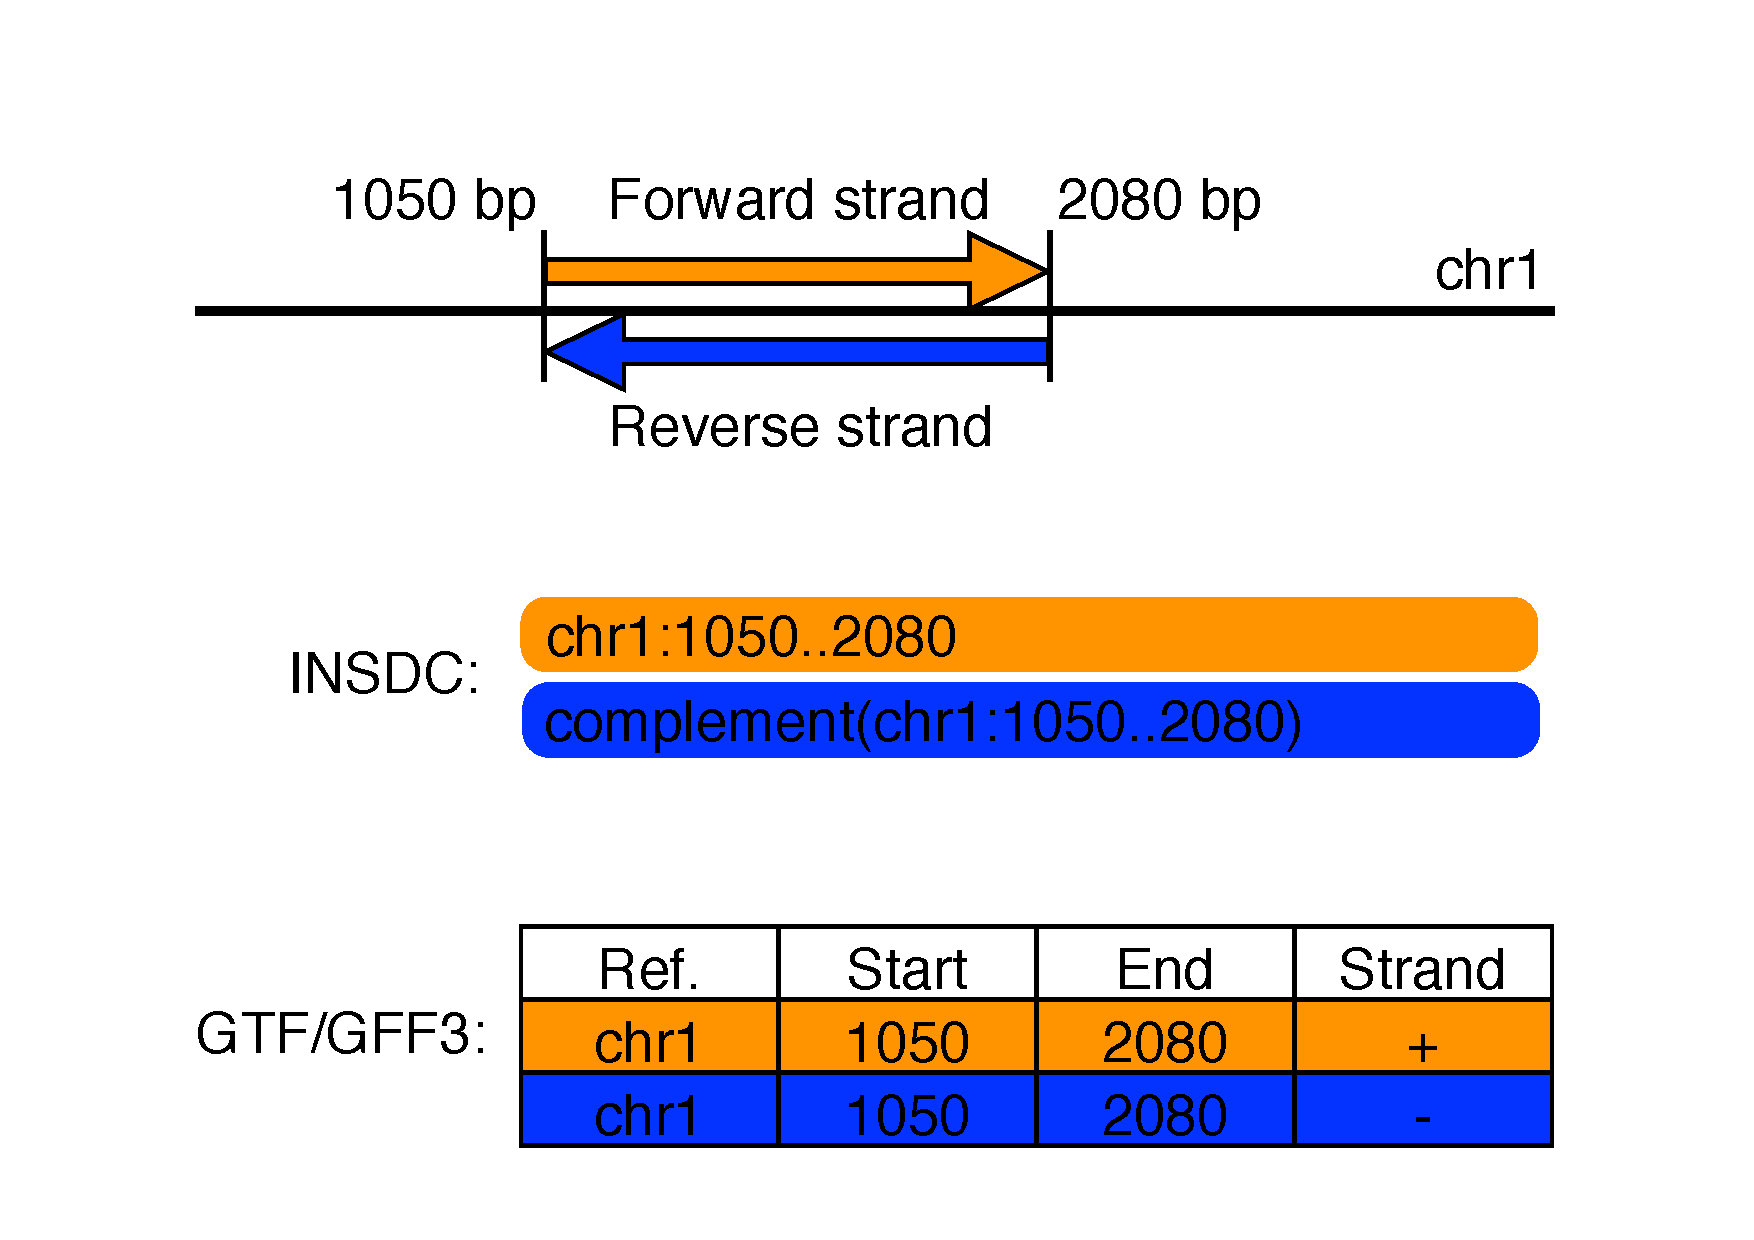
\includegraphics[width=10cm]{figures/figure-strand.pdf}
\end{center}
\caption{Assorted conventions for regions, start, end, and strands.
This figure shows two hypothetical features on a DNA sequence
(labelled \texttt{chr1}), on either the forward strand (orange) or
reverse strand (blue).
Using the INSDC location string notation, these regions are
``\texttt{1050..2080}'' and ``\texttt{complement(1050..2080)}''
respectively if implicitly given in terms of the reference chr1.
Using the GTF/GFF3 family of formats, regardless of the
strand these two locations are described with $start = 1050$
and $end = 2080$, and in general, $start \leq end$.
Biologically speaking, in terms of transcription, the start of a genomic
feature is strand dependent.
For the forward strand feature (orange), the start is 1050
while the reverse strand feature (blue) starts from 2080.
\textit{TODO - Replace with real example? Add FALDO illustration?}
}
\label{fig:strands}
\end{figure}
